%18/11 - Dido Carrero
\part{Variantes genómicas: técnicas, llamada de variantes y anotación}
\chapter{Introducción a las variantes germinales}
\section{Análisis genómico}
El análisis genómico incluye varios pasos: primero, la extracción de muestras y la preparación de las librerías; luego, la secuenciación, el control de calidad de los archivos FastQ (donde se descartan las lecturas con errores, ya que una mayor refinación del pipeline implica un control de calidad más estricto); el alineamiento de las lecturas; la identificación o llamada de variantes (SNP, INDEL, CNV, SV); la anotación de los archivos VCF; la visualización de las variantes candidatas y, finalmente, los pasos de priorización y filtrado.

En general, en un análisis de genoma, pueden encontrarse muchas variantes en comparación con el genoma de referencia, por lo que es necesario aplicar filtros para identificar aquellas que sean realmente relevantes a nivel clínico. La validación final se realiza en el laboratorio mediante PCR.

Las variantes germinales se originan en la línea germinal, es decir, en los gametos, lo que las hace heredables y presentes en todo el organismo. En cambio, las variantes somáticas ocurren en células que no pertenecen a los gametos, son mutaciones adquiridas durante la vida y afectan solo a un linaje celular específico.

En la práctica, ya sea que se realice un análisis somático o germinal, se extraen muestras tanto del tejido tumoral como del tejido sano. Si se sospecha de una enfermedad genética germinal, también se debe extraer una muestra de un tejido germinal.

La frecuencia alélica es la proporción de moléculas de ADN en la muestra que contienen una mutación específica. Se calcula mediante la siguiente fórmula:
$$VAF = \frac{sequence.reads.with.a.DNA.variant}{overall.coverage.at.that.locus}$$
Este número es clave para diferenciar una variante somática de una germinal. En un organismo diploide, un locus heterocigoto debería mostrar un VAF cercano a 0,5, un locus homocigoto tendrá un VAF de 1 y un locus de referencia tendrá un VAF de 0. Las variantes somáticas presentan una frecuencia alélica muy variable, mientras que las variantes germinales suelen tener valores de VAF de 0, 0,5 o 1, dependiendo de si están presentes en uno, ambos o ninguno de los alelos.

\subsection{GATK}
GATK es un conjunto de herramientas desarrollado por el Broad Institute para el análisis de variantes genómicas. A partir de archivos BAM, estas herramientas permiten realizar un análisis completo de variantes. El paquete incluye buenas prácticas y un flujo de trabajo (workflow) que varía dependiendo de si se analizan variantes germinales o somáticas.

\begin{figure}[h!]
\centering
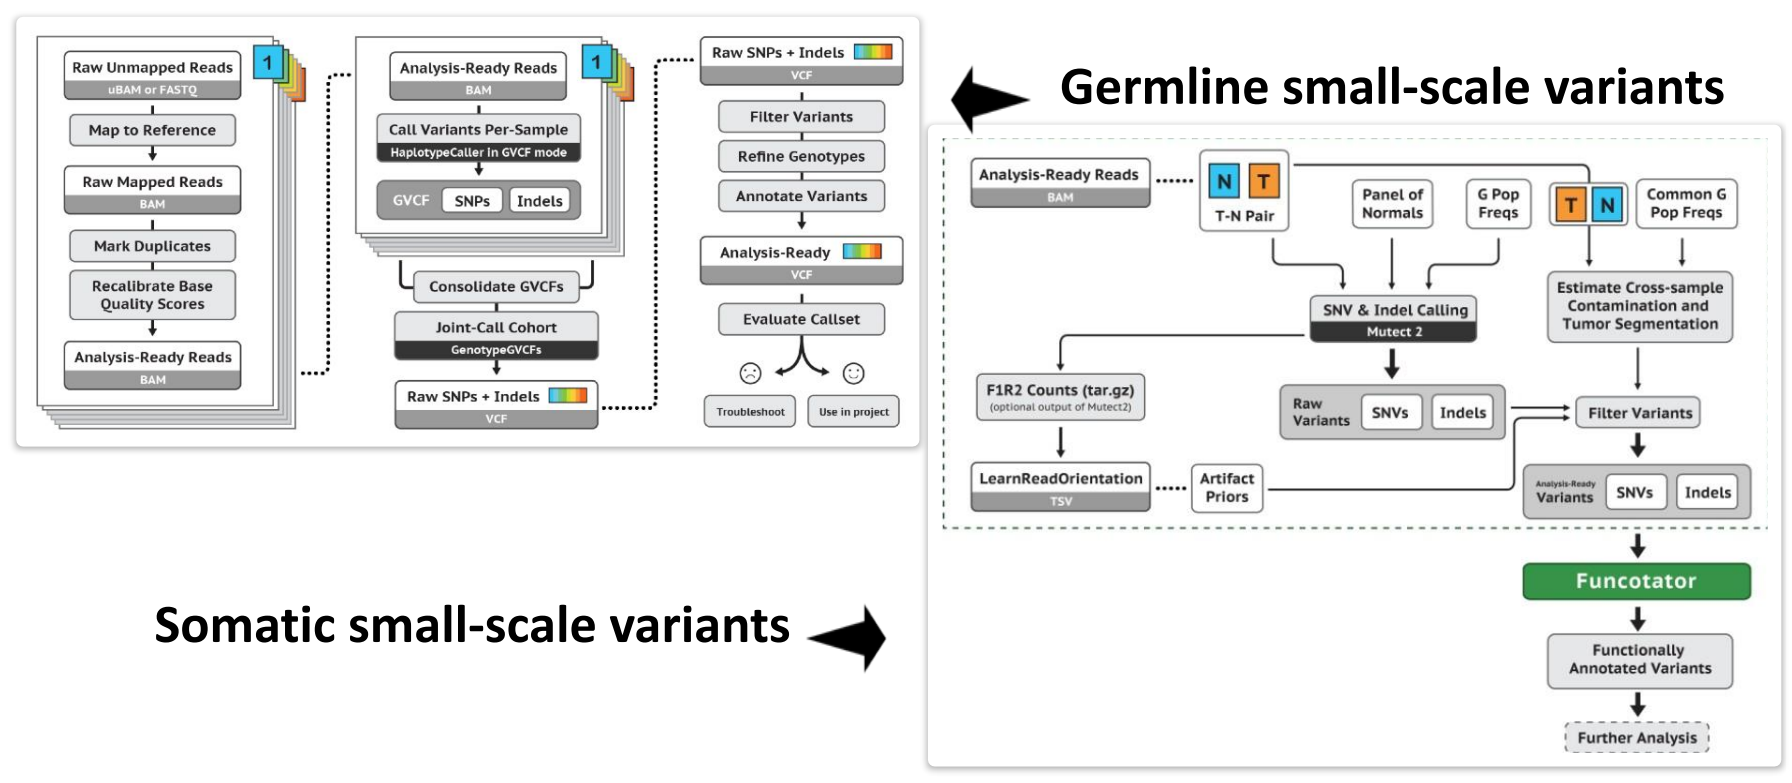
\includegraphics[width = 0.8\textwidth]{figs/gatk-pipelines.png}
\end{figure}

HaplotypeCaller es una herramienta utilizada para la llamada de variantes, basándose en el cálculo de la probabilidad de los genotipos. Utiliza un archivo BAM como entrada y produce un archivo de salida en formato VCF o GVCF con los genotipos 1/1, 0/1 y 0/0. Este archivo VCF debe ser filtrado mediante recalibración de bases (una práctica recomendada) o mediante hard-filtering. Si el archivo de salida es un GVCF, será necesario realizar un paso intermedio antes de aplicar el filtro y continuar con el análisis posterior. Además, con la opción -ploidy, se puede especificar la ploidía del organismo.

El comando básico para la herramienta es:
\begin{lstlisting}[language = bash]
gatk HaplotypeCaller \
	-R reference.fasta \
	-I preprocessed_reads.bam \
	-O germline_variants.vcf
\end{lstlisting}

MuTect2 es una herramienta diseñada para la llamada de variantes somáticas. Permite detectar SNVs e INDELs, con frecuencias alélicas variables, y es capaz de diferenciar entre variantes somáticas y germinales. MuTect2 ofrece varios modos: tumor con normal emparejado, solo tumor o modo mitocondrial.

\section{Práctica: análisis de datos}
Vamos a recibir los datos de cáncer de mama. Se ha secuenciado todo el exoma con Illumina. Primero creamos el entorno conda \texttt{OVCA\_case}. 
\begin{lstlisting}[language=bash]
conda create -n OVCA_case
conda activate OVCA_case
conda install bioconda::gatk4
conda install bioconda::samtools
\end{lstlisting}

Con los datos descargados, utilizamos la herramienta HaplotypeCaller. Lo primero que debemos hacer es realizar los índices de la referencia y del fichero bam:
\begin{lstlisting}[language=bash]
samtools dict  REFERENCE/hg19_chr17.fa -o  REFERENCE/hg19_chr17.dict
samtools faidx REFERENCE/hg19_chr17.fa
samtools index bams/normal_refined.bam
\end{lstlisting}

A continuación utilizamos la herramienta:
\begin{lstlisting}[language=bash]
gatk HaplotypeCaller -R REFERENCE/hg19_chr17.fa -I bams/normal_refined.bam -O out/normal_refined_out.vcf
\end{lstlisting}

El fichero resultante empieza con una cabecera con dos almohadillas y el cromosoma de referencia. Se muestra la información acerca de la generación del fichero y los filtros. Con una almohadilla se muestra el significado de cada columna: cromosoma en el que está la variante, posición genómica, ID, alelo de referencia, alelo alternativo con la mutación encontrada, score de calidad, filtros, información adicional con la anotación, formato del siguiente campo y normal. Dentro del formato, se distinguen: GT indica el genotipo, AD el número de lecturas que soporta la variante (en formato referencia,variante) y DP el total de lecturas.

El siguiente paso es la recalibración de variantes. Muchas veces, la calidad de las variantes que aparece de manera directa (columna QUAL) se debe recalibrar. Este modelo puntúa las calidades de las variantes y filtrar aquellas que no pasen los filtros. Se comprueba que una variante sea efectivamente verdadera. Para ello, se da un archivo de referencia de variantes y se estima si la variante es un artefacto de la secuenciación o una variante de verdad. El resultado es VQSLOD, que se añade al campo de información. Esto en general se realiza para SNPs e INDELs por separado debido a que las bases de datos de variantes son diferentes. 

El paso siguiente es aplicar los filtros VQSR. En la columna FILTER anota si la variante pasa filtros o no, pero no descarta aquellos que no pasen los filtros; si se quiere eso se debe especificar.
\begin{lstlisting}[language=bash]
tabix -p vcf Annotations/dbsnp_138.hg19_chr17.vcf.gz

gatk VariantRecalibrator -R REFERENCE/hg19_chr17.fa -V out/normal_refined_out.vcf
--resource:dbsnp,known=true,training=true,truth=true,prior=15.0
Annotations/dbsnp_138.hg19_chr17.vcf.gz -an QD -an ReadPosRankSum -an FS -an SOR -mode BOTH -O out/output_normal_refined.recal --tranches-file out/output_normal_refined.tranches

gatk ApplyVQSR -R REFERENCE/hg19_chr17.fa -V out/normal_refined_out.vcf -O out/output_normal_refined.recalibrated --truth-sensitivity-filter-level 99.0 --tranches-file out/output_normal_refined.tranches --recal-file out/output_normal_refined.recal -mode BOTH
\end{lstlisting}

El último paso es el filtrado de las variantes. 
\begin{lstlisting}[language=bash]
awk -F '\t' '{if ($0 ~ /#/ || $7 == "PASS") print}' out/output_normal_refined.recalibrated > out/output_normal_refined.onlypass

#Contar el número de líneas resultantes
grep "^chr17" out/output_normal_refined.onlypass | wc -l
\end{lstlisting}

%21/11 - Dido
\chapter{Introducción a las variantes somáticas}
\section{Control de calidad y refinamiento de alineamientos}
\subsection{Control de calidad}
Los controles de calidad se suelen hacer en varios puntos de todo el proceso. Hay varios puntos clave, y después de cada uno de ellos se realiza el control de calidad. El primero y más importante parte de los archivos FastQ de secuenciación, ya que si éstos están mal, el resto del análisis carece de sentido.

Se utiliza el programa FastQC que da un informe en HTML con varias estadísticas de los archivos. Hay otros programas que se pueden utilizar, como samtools, que indica si hay secuencias duplicadas y otras estadísticas. MultiQC combina varias herramientas para sacar un informe completo.

En los controles de calidad, se mira si hay un número de lecturas dentro del rango esperado, si las bases tienen una buena calidad mediante el Phred score, y si hay contaminación en las muestras. Una secuencia que aparezca repetidamente puede ser muy repetitiva en el genoma que se secuencie o una contaminación.

FastQC permite visualizar la calidad por base por secuencia, el contenido GC y secuencias sobrerrepresentadas entre otras métricas, pero esas son las que habitualmente están mal. En cuanto a la evaluación de la calidad por base, se ve la distribución de los scores en las lecturas. En secuenciación de Illumina, es habitual que al final de las lecturas la calidad decaiga un poco, pero debería seguir en un rango elevado. Si la calidad decae mucho, se trata de un error en la secuenciación. En los scores por secuencia, se espera que la mayoría de las secuencias tengan una puntuación muy alta. Si hay varias secuencias con una calidad baja, eso indica que algo está mal, pero es difícil indicar la causa (problema del secuenciador, purificación de las muestras, contaminación, librería, etc). La distribución esperada del contenido en GC debería seguir una distribución normal, aunque hay veces que se puede desviar un poco.

\begin{lstlisting}[language=bash]
conda install bioconda::fastqc
fastqc -o out/ Raw_data/*.fastq
\end{lstlisting}

El resultado es un fichero html y zip por cada FastQ. En cuanto a Normal R1, el contenido GC muestra un mensaje de error. Hay un pico muy grande alrededor del 60\%, cuando en humanos debería rondar el 50\%. Además, hay varias lecturas con un contenido GC bajo, sobre el 35\%. Como estos resultados son malos, se puede valorar descartarlos y repetir la secuenciación, pero en laboratorios pequeños puede ser un problema. Además, tenemos una secuencia sobrerrepresentada de N, que no nos preocupa porque se va a descargar. Todas las demás métricas han salido bien. En Normal R2, las secuencias sobrerrepresentadas dan error, pero sigue siendo una secuencia de todo N, por lo que se le puede dar poca importancia. El contenido GC también da error. En cuanto a las muestras de tumor, son muy similares: tienen un contenido GC más bajo y tiene una secuencia de N sobrerrepresentada. 
Hay que tener en cuenta que estamos trabajando solo con el cromosoma 17, pero que la distribución esperada está calculada sobre todo el genoma. Por tanto, si ese cromosoma tiene muchas secuencias repetitivas en AT, ya de por sí habrá un sesgo en la comparación con la distribución esperada. 

\subsection{Alineamiento}
En cuanto al alineamiento, se utiliza BWA. Se puede utilizar la siguiente chuleta para la indexación en base al fichero que se tenga:
\begin{lstlisting}[language=bash]
#Fasta
bwa index reference.fasta
samtools dict reference.fasta -o reference.dict
samtools faidx reference.fasta

#BAM
samtools index bam.file

#VCF
tabix -p vcf vcf.file
\end{lstlisting}

El siguiente paso es la alineación.
\begin{lstlisting}[language=bash]
bwa mem -R '@RG\tID:OVCA\tSM:Normal' REFRENCE/hg19_chr17.fa Raw_data/WEx_Normal_R1.fastq Raw_data/WEx_Normal_R2.fastq > alignment/normal.sam
bwa mem -R '@RG\tID:OVCA\tSM:Tumour' REFRENCE/hg19_chr17.fa Raw_data/WEx_Tumour_R1.fastq Raw_data/WEx_Tumour_R2.fastq > alignment/tumour.sam
\end{lstlisting}

Se puede utilizar \texttt{samtools flagstat normal.sam} para ver unas estadísticas como alineamientos mapeados, primarios, secundarios, duplicados, etc. 

\subsection{Refinamiento del alineamiento}
En este paso, queremos convertir los SAM en BAM para que los ficheros estén comprimidos y binarizados. Además, BWA a veces omite alguna información en los ficheros SAM que queremos rellenar.
\begin{lstlisting}[language=bash]
samtools fixmate -O bam alignment/normal.sam alignment/normal_fixmate.bam
samtools fixmate -O bam alignment/tumour.sam alignment/tumour_fixmate.bam
\end{lstlisting}

Los duplicados vienen de la amplificación por PCR durante la preparación de la librería. Un error al principio de la PCR se propaga. Los duplicados en secuenciación híbrida no aportan nada al análisis posterior, pudiendo dar lugar a falsos positivos y redundancia. Por ello, lo mejor es descartar estas duplicaciones. Además, para la llamada de variantes es necesario que el alineamiento esté ordenado por posición genómica, y aprovechamos para indexar el BAM.
\begin{lstlisting}[language=bash]
samtools sort -O bam -o alignment/normal_sorted.bam alignment/normal_fixmate.bam
samtools sort -O bam -o alignment/tumour_sorted.bam alignment/tumour_fixmate.bam

samtools rmdup -S alignment/normal_sorted.bam alignment/normal_refined.bam
samtools rmdup -S alignment/tumour_sorted.bam alignment/tumour_refined.bam

samtools index alignment/normal_refined.bam
samtools index alignment/tumour_refined.bam
\end{lstlisting}

Con esto hemos creado los bams que utilizamos en la parte anterior de las variantes germinales. Se pueden eliminar los ficheros intermedios de ficheros sam, fixmate y sorted, dejando los bam refinados.

\section{Recalibración de la calidad de base}
Cada posición de la secuencia tiene su calidad de base. Las diferentes tecnologías NGS tienen sus sesgos dependiendo del contexto, por lo que es importante hacer la recalibración para corregir empíricamente esos sesgos. La recalibración de bases no es lo mismo que la recalibración de variantes (eso viene después con los VCF).

La recalibración de bases consta de dos pasos. Primero, BaseRecalibrator parsea las lecturas y crea una tabla en la que se asigna a cada lectura el ciclo durante el que se leyó la base, su puntuación y la puntuación de las bases que van antes y después. EL modelo computa cuántas veces hay un cambio en la referencia según dbSNP, excluyendo los loci de alta variabilidad. Después, la herramienta ApplyBQSR parsea las lecturas y, utilizando la matriz de antes, recalibra las puntuaciones. Así, las calidades son más similares a las puntuaciones empíricas, pudiendo utilizarse para el variant calling.

\section{Llamada de variantes somáticas}
Las variantes son cambios permanentes en el ADN de un organismo que pueden deberse a errores durante la replicación, durante la recombinación durante la formación de gametos y por factores externos como radiación, viruses, transposones, rayos ultravioleta, etc. El genoma entre humanos es idéntico en un 99,9\%. El 0,1\% restante es la fuente de variabilidad, permitiendo los mecanismos de evolución, las diferencias fenotípicas entre individuos y en la respuesta a enfermedades y fármacos. 

\begin{figure}[htbp]
\centering
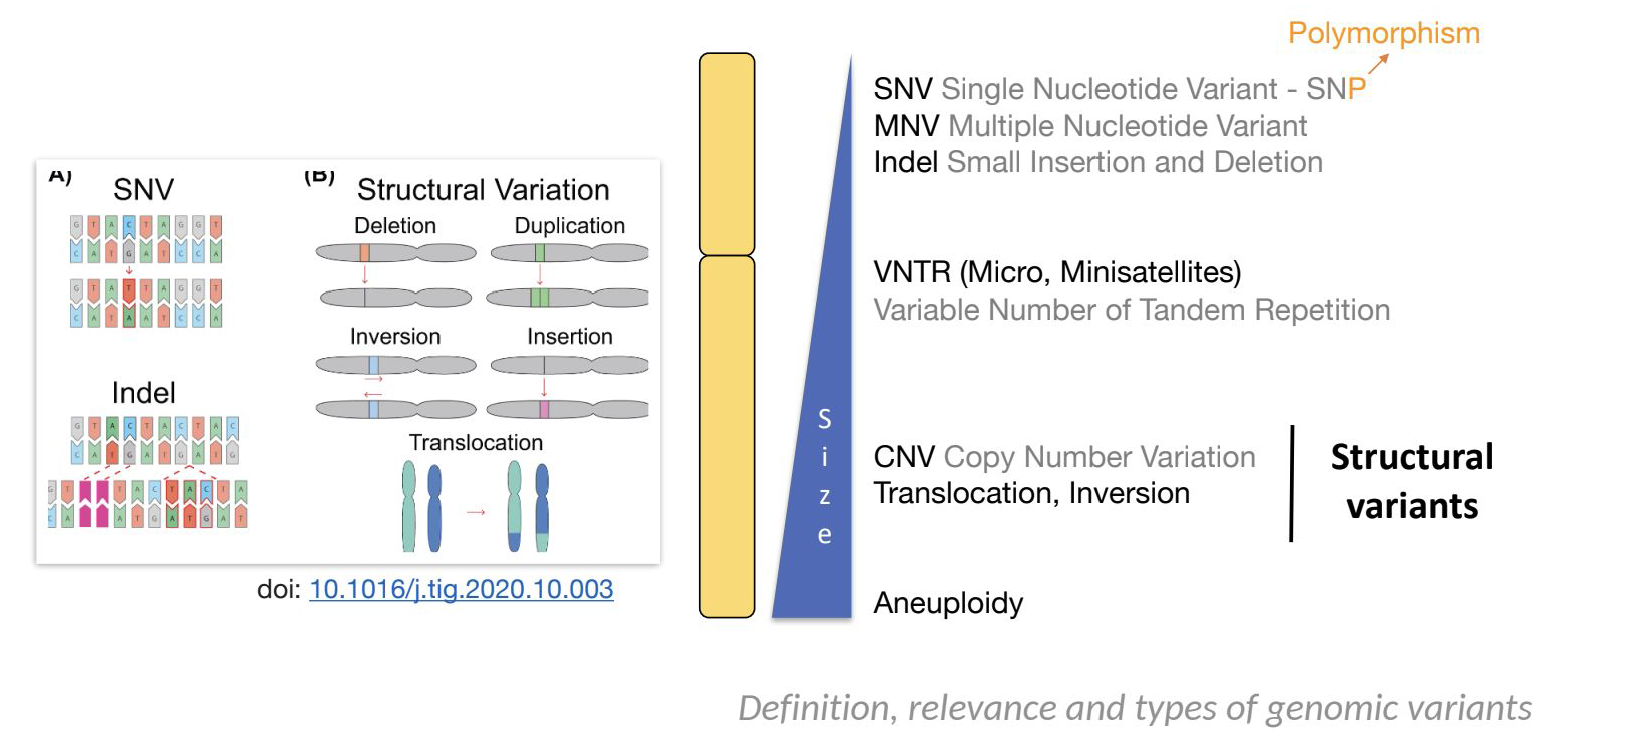
\includegraphics[width = \textwidth]{figs/variants-size.png}
\end{figure}

En función de la posición de la secuencia, puede haber variantes intergénicas (entre genes) en secuencias reguladoras o upstream o downstream de algún gen en concreto. Dentro de genes, puede haber variantes en las regiones UTR, en los exones, en los intrones o en regiones de splicing. 

Para realizar la llamada de variantes, se utiliza MuTect2. Es similar a GATK, pero permitiendo mayor variabilidad de frecuencia alélica (no solo 0, 0,5 y 1 como GATK), además de evitar las variantes germinales. Hay distintos modos: tumor con tejido normal (este es el óptimo), solo tumor y mitocondrial. Se crea un panel de normales para poder inferir qué mutaciones son exclusivamente somáticas. 
\begin{lstlisting}[language=bash]
#Modo Tumor-only 
gatk Mutect2 -R REFERENCE/hg19_chr17.fa -I alignment/tumour_refined.bam -O tumour_only_somatic.vcf

#Modo tumor with matched normal
gatk Mutect2 -R REFERENCE/hg19_chr17.fa -I alignmetn/tumour_refined.bam -I alignment/normal_refined.bam -normal Normal -O out/tumour_matched_somatic.vcf
\end{lstlisting}
 
Después del filtrado, obtenemos las siguientes variantes somáticas:
\begin{lstlisting}[language=bash]
grep "^chr17" out/tumour_matched_somatic.vcf | wc -l #193
grep "^chr17" out/tumour_only_somatic.vcf | wc -l #461
\end{lstlisting}
Cuando solo se mide el tumor, el número es casi el doble. Al dar el normal, el algoritmo sabe qué variantes son germinales por estar ya presentes en el tejido y los descarta. Al medir solo el tumor, algunas variantes germinales se excluyen, pero otras se cuelan, por lo que el número de variantes es mayor. 

Las frecuencias alélicas vienen en la columna FORMAT bajo AF. Estas frecuencias van del 0 al 1 en todo el rango. En las variantes germinales, esta información aparece en INFO y es de 0, 0,5 o 1.